\documentclass[12pt,letterpaper,titlepage]{article}

\usepackage{fontspec}
\defaultfontfeatures{Mapping=tex-text}
\usepackage{xunicode}
\usepackage{xltxtra}
\usepackage{amsmath}
\usepackage{pdfpages}
\usepackage{amsfonts}
\usepackage{bbold}
\usepackage{amssymb}
\setcounter{secnumdepth}{0}
\usepackage{nameref}
\usepackage{enumitem}
\usepackage{environ}
\usepackage{pgfplots}
\usepackage{listings}

\showboxdepth=\maxdimen
\showboxbreadth=\maxdimen


\usepackage{paracol}
\usepackage{wrapfig}
\globalcounter{table}
\globalcounter{figure}
\usepackage{graphicx}
\usepackage[left=1in,right=1in,top=1in,bottom=1in]{geometry}
\graphicspath{{img/}}

\author{Jacob Abel}
\title{	Design \& Simulate 9
	\\\large ECE2204 CRN:82929
}

\setlength{\parskip}{0.5em}

\begin{document}
\maketitle
\begin{raggedright}

\section{Problem 9.2-3.a.1: } 
\subsection{Design}

The circuit below takes a 120V(rms) 60Hz AC input and outputs a positive rectified DC current. Redesign the circuit to output an output voltage of $V_O = -12V$, a ripple voltage of $V_r = 0.05V$, and use diodes with $V_\gamma=1.2V$. Assume an output load resistance of $R_L = 17k\Omega$

\begin{center}
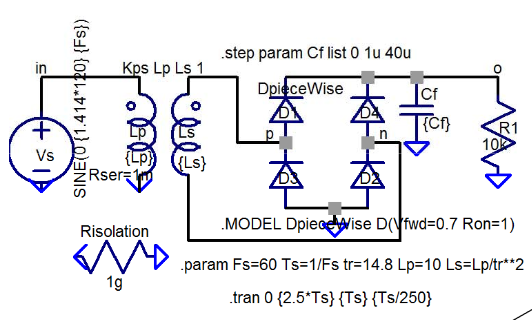
\includegraphics[width=\textwidth, height=12\baselineskip, keepaspectratio=true]{ds1}
\end{center}

\begin{align*}
    V_S{max} 
      &= |V_O(max)| + 2V_\gamma
       = |12V| + 2 \times 1.2V
       = 14.4V
\\  V_{Srms}
	  &= \frac{14.4V}{\sqrt{2}}
	   = 10.18V
\\  Tr
	  &= \frac{120V}{10.18V}
	   = 11.79
\\  PIV
	  &= V_S(max) - V_\gamma 
	   = 14.4V - 1.2V
	   = 13.2V
\\  Cf
      &= \frac{V_M}{2fRV_r}
       = \frac{12V}{2(60Hz)(17k\Omega)(0.05V)}
       = 0.118mF
\end{align*}

\clearpage
\subsection{Validation}

\begin{center}
LTSpice Implementation (values within $<1\%$)
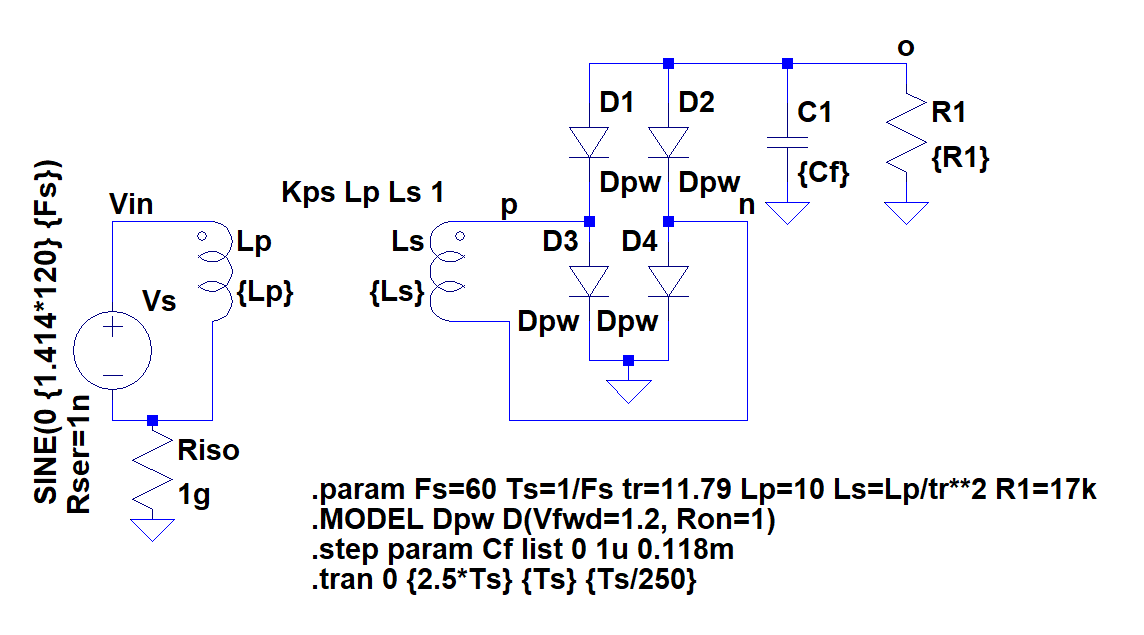
\includegraphics[width=.8\textwidth, height=\textheight, keepaspectratio=true]{ds1b}

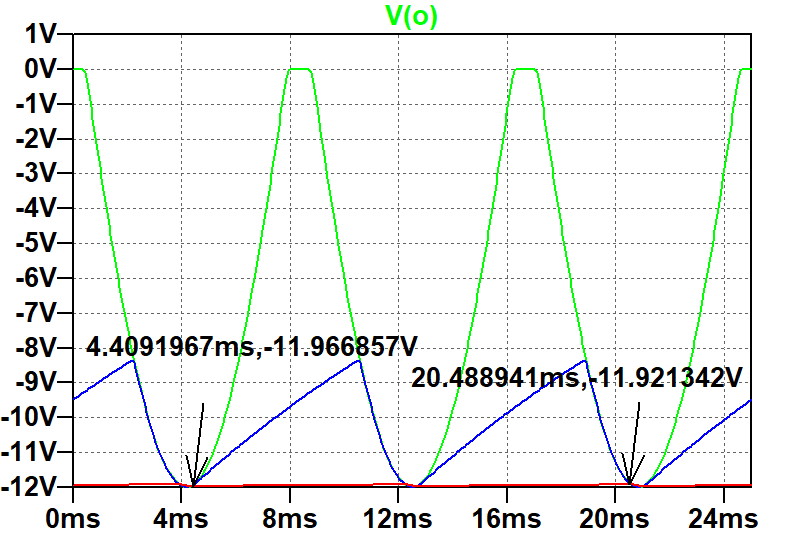
\includegraphics[width=.7\textwidth, height=\textheight, keepaspectratio=true]{ds1c}

$V_r = |-11.967V+11.921V| = \pm0.041V$

Simulated $V_r$ is within the required $\pm0.05V$. 

$Err_{V_O} = \frac{12V-11.967V}{12V} = 0.0028 = 0.28\%$
\end{center}

\clearpage
\section{Problem 8.2-5.b.1: }
\subsection{Design}

Convert the prior problem into a center tapped transformer DC rectifier.

\begin{align*}
    V_S{max} 
      &= |V_O(max)| + V_\gamma
       = |12V| + \times 1.2V
       = 13.2V
\\  V_{Srms}
	  &= \frac{13.2V}{\sqrt{2}}
	   = 9.33V
\\  Tr
	  &= \frac{120V}{9.33V}
	   = 12.86
\\  PIV
	  &= V_S(max)
	   = 13.2V
\\  Cf
      &= \frac{V_M}{2fRV_r}
       = \frac{12V}{2(60Hz)(17k\Omega)(0.05V)}
       = 0.118mF
\end{align*}


\clearpage
\subsection{Validation}

\begin{center}
LTSpice Implementation (values within $<1\%$)

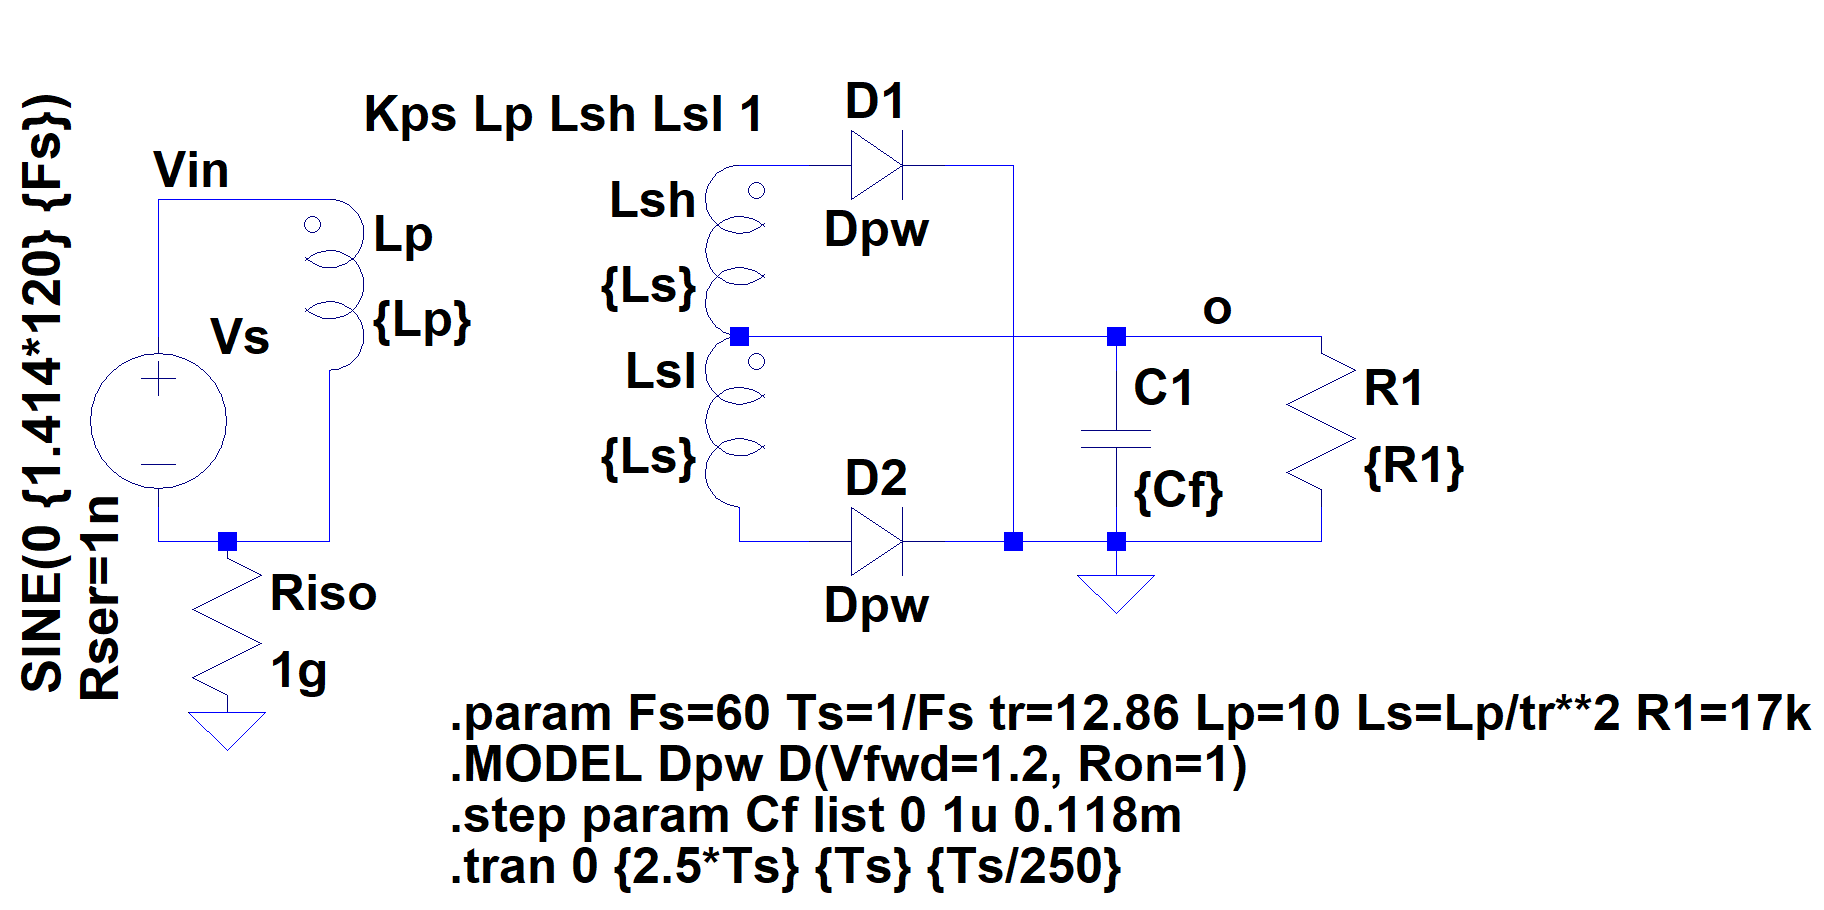
\includegraphics[width=.75\textwidth, height=\textheight, keepaspectratio=true]{ds2b}

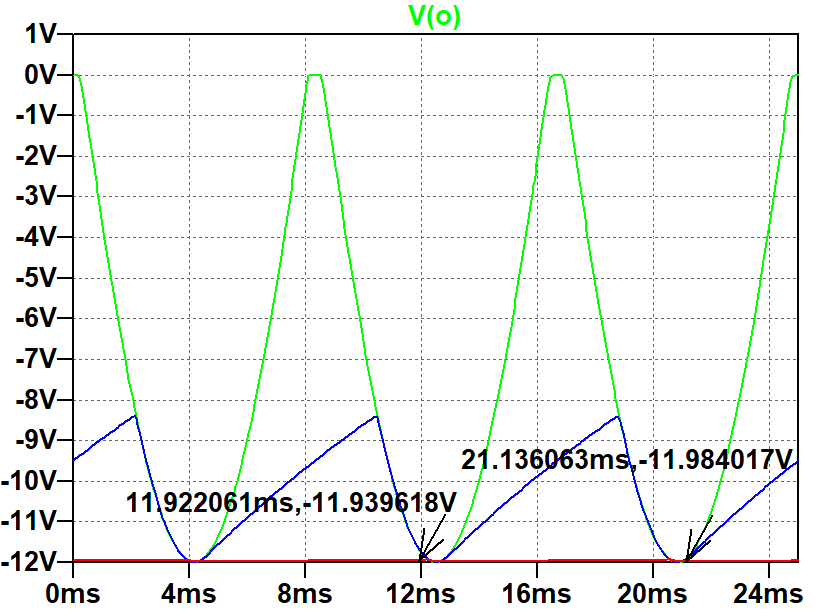
\includegraphics[width=.65\textwidth, height=\textheight, keepaspectratio=true]{ds2c}

$V_r = |-11.984V+11.939V| = \pm0.050V$

Simulated $V_r$ is exactly at the specified $\pm0.05V$. 

$Err_{V_O} = \frac{12V-11.984V}{12V} = 0.0028 = 0.28\%$
\end{center}

This assignment should demonstrate a basic understanding of using filter and rectifier circuits.

\textit{I have neither given nor received unauthorized assistance on this assignment.}


\end{raggedright}
\end{document}
